\documentclass[12pt]{article}

\usepackage[left=.6in, right=.6in, top=0.75in, bottom=0.75in]{geometry}
\setlength\parindent{0pt}

\usepackage{graphicx, amsmath,anonchap,tabularx, multicol,array,graphbox}
\usepackage{cancel}
\usepackage{enumitem}
\setlist{noitemsep}
\setlist{nolistsep}
\usepackage{float}
\usepackage{multicol}
 
%\usepackage{draftwatermark}
%\SetWatermarkText{DRAFT}
%\SetWatermarkScale{5}
%\SetWatermarkColor[rgb]{0.8,0.8,0.8}
\newenvironment{boxe}
    {\begin{center}
    \begin{tabular}{|p{0.9\textwidth}|}
    \hline\\
    }
    { 
    \\\\\hline
    \end{tabular} 
    \end{center}
    }
    
\begin{document}

\begin{tabular*}{\textwidth}{@{\extracolsep{\fill}}l l}

\textbf{Math 160, Optimization}   \\
\end{tabular*} \\

\begin{enumerate}
    \item Use the first derivative test to find the local minimums/maximums of the function 
    $q(x)=\displaystyle{\frac{x^2+5}{x-2}}$ 
    \begin{itemize}
        \item[(a)] Compute $q'(x)$\\\\\\\\
        \item[(b)] Where is $q'(x)$ undefined? (Think about what values of $x$ result in dividing by zero)\\\\\\\\
        \item[(c)] Where is $q'(x)=0$ (Hint: If the numerator of $q'(x)$ then $q'(x)$ is zero. 
        It is enough to only look for when the numerator is zero)\\\\\\\\\\\\\\\\\\\\
        \item[(d)] Find the points of interest and the critical points of $q(x)$.\\\\\\\\
        \item[(e)] Create a first derivaitve sign chart and then use the first derivative test to classify your critical points as local min or max or neither.\\\\\\\\\\
    \end{itemize}
\newpage
    \item (a) Verify that $f(x)=\sin(x^2-x)$ has a local minimum at $x=1/2$ using the second derivative test.\\
    
    \vspace{4in}

    (b) Does $f(x)$ have a local max at $x=1$?

\iffalse
    \item Let $f(x)$ be a continuous function with the following properties
    \vspace{-.16in}
	\begin{itemize}
	\begin{multicols}{2}
	\item $f(-3)=-2$
	\item $f(0)=3$
	\item $f(1)=0$
	\item $f'(-3)=0$
	\item $f'(0)=0$
	\item $f'(1)$ is undefined
	\item $f'(x)<0$ for $-\infty<x<-3$, $0<x<1$
	\item $f'(x)>0$ for $-3<x<0$ and $1<x<\infty$
	\item $f''(x)<0$ for $1<x<4$ and $-1<x<1$ 
	\item $f''(x)>0$ for $4<x<\infty$ 
	\end{multicols}
	\end{itemize}
    (a) Find the critical points of $f$.\\\\\\\\\\
    (b) Using the Second Derivative Test, classify each as a local min/max or 
    explain why the test is inconclusive and then use the First Derivative Test.\\\\\\\\\\
    (c) Sketch the graph of a continuous 
    function having the following properties:

	\begin{center}
	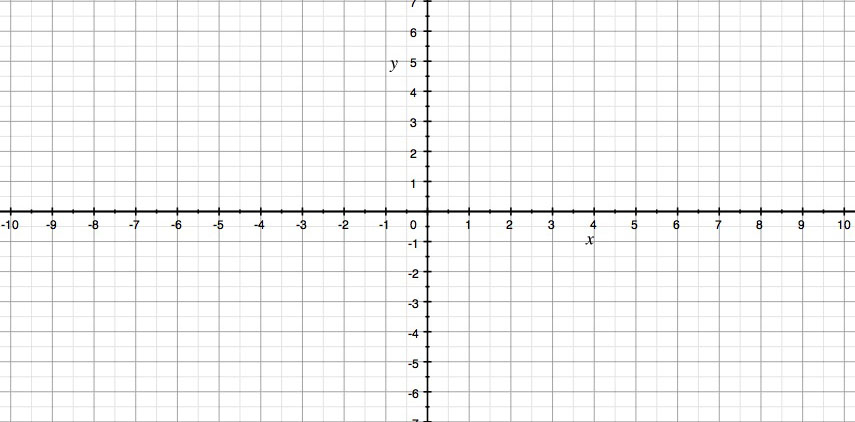
\includegraphics[scale=0.5]{Axes2a.jpg}\end{center}
    \fi
    \newpage
    \item Consider the function $f(x)=x^3-ax$ on the interval $[-3,2]$ where $a$ is a constant.
    \begin{itemize}
        \item Find the critical points of $f(x)$ in terms of $a$.\\\\\\\\\\
        \item Will $f(x)$ always have a global maximum and minimum?\\\\\\
        \item Find a value for $a$ such that there is a global maximum at $x=-2$.\\\\\\\\\\\\\\\\\\
        \item Find a value for $a$ such that there is a global maximum at $x=2$.\\\\\\\\\\\\
        \item T/F: There is a value for $a$ such that there is a global maximum at $x=0$. (Hint: Can $x=0$ be a critical point? When it is, can it also be a local minimum or maximum?)
    \end{itemize}
    %\item Find the global maximum and minimum of the function $\displaystyle{f(t)=\frac{t}{1+t^2}}$ on $(-\infty,\infty)$ or explain why they don't exist. Hint: EVT does not apply here, why? How could looking at the end behavior help?\\
    
    \vspace{4in}

    \newpage
    \item You have $300$ft of fencing and you are trying to build a rectangular pen for your goats against the side of a barn (such that one side of the pen will be the barn). How can you maximize the area of the pen (find dimensions for the pen that maximizes the area)? Assume that the barn is as big as needed.
    \begin{itemize}
        \item Draw a picture of the situation above and assign variable to all quantities. And indicate what quantity needs to be maximized or minimized?\\\\\\\\\\\\\\\\\\\\\\

        \item Write a general equation for the quantity you are maximizing or minimizing in terms of one variable. (Hint: use the constraints from the problem).\\\\\\\\

        \item Now that you have an equation. Find an interval for you input variable that makes sense for your problem. \\\\
        
        \item Find the critical points of your function.\\\\\\\\\\\\\\\\\\

        \item Now using the critical points find the maximum or minimum value of your function (don't forget to check the endpoints).\\\\\\\\\\

        \item Now use what you have found to answer the original questions.
    \end{itemize}
    \newpage
    \item You are in charge of building a rectangular storage container with an open top and a volume of $10\ m^{3}$. The base of the box has to be twice as long as it is wide. It costs \$30 per $m^{2}$ to construct the base and \$32 per $m^{2}$ to construct the sides. Call the length, width, and height of the box $l$, $w$, and $h$, respectively. What are the dimensions to create the least expensive box?
    \begin{itemize}
        \item Draw a diagram of this situation and label all quantities.\\\\\\\\\\\\\\\\
        \item What are the unknowns and knows in this scenario? What is being optimized? Is this a minimization or maximization problem?\\\\\\


        \item Write an equation for the area of the base in terms of $w$.\\\\\\
        
        \item Write an equation for the area of all the sides in terms of $w$ and $h$.\\\\\\

        \item Write an equation for the volume of the box in terms of $w$ and $h$.\\\\\\

        \item Rewrite the cost $C$ is terms of only $w$, call this $C(w)$. Is there an interval for $w$ for this problem? Does EVT apply here?\\\\\\\\

        \item Find the critical points of $C(w)$.\\\\\\\\\\\\\\\\
        
        \item Find the absolute minimum of $C(w)$ and verify it is in fact a minimum. What are the dimensions of the box?
    \end{itemize}

    \newpage
    \item You are planning to connect a small island with fiber optic cables to the fiber optic internet grid. The island is 14 miles off of a straight coastline and the nearest point on the grid is 10 miles down the coast from the point directly opposite the island. Laying underwater cables cost twice as much as laying cables on land. Use calculus to solve and justify your work for the questions below. Round mileage values to at least \textbf{4 decimal places}, and round dollar values to \textbf{2 decimal places}.
    \begin{enumerate}[label=(\alph*)]
        \item Which combination of underwater and land-based cable will minimize the total cost of the cable? What is the minimum cost if the cable costs $\$50,000$ per mile on land?

        \vspace{4in}
        
        %\item What would happen to your result if the nearest point on the grid from problem 6a were $20$ miles down the coats rather than $10$ miles?
        \newpage
        \item Assume again that the nearest point on the grid was $10$ miles down the coast. Suppose that the underwater cable costs $\alpha$ times as much as cable on land ($\alpha>1$). Which combination of the underwater and land-based cable will minimize the total cost of the cable now? (write your answer in terms of $\alpha$). Interpret your answer.
    \end{enumerate}
\vspace{7in}
\item Challenge question: Find the volume of the largest right circular cone that can be inscribed in a sphere of radius $3$. Google definitions and formulas as needed.

        
    
\end{enumerate}


\end{document}
